%!TEX root = ../dissertation.tex
%\begin{savequote}[75mm]
%\qauthor{Quoteauthor Lastname}
%\end{savequote}

%% Set up problem
\begin{figure*}[t]
\begin{center}
{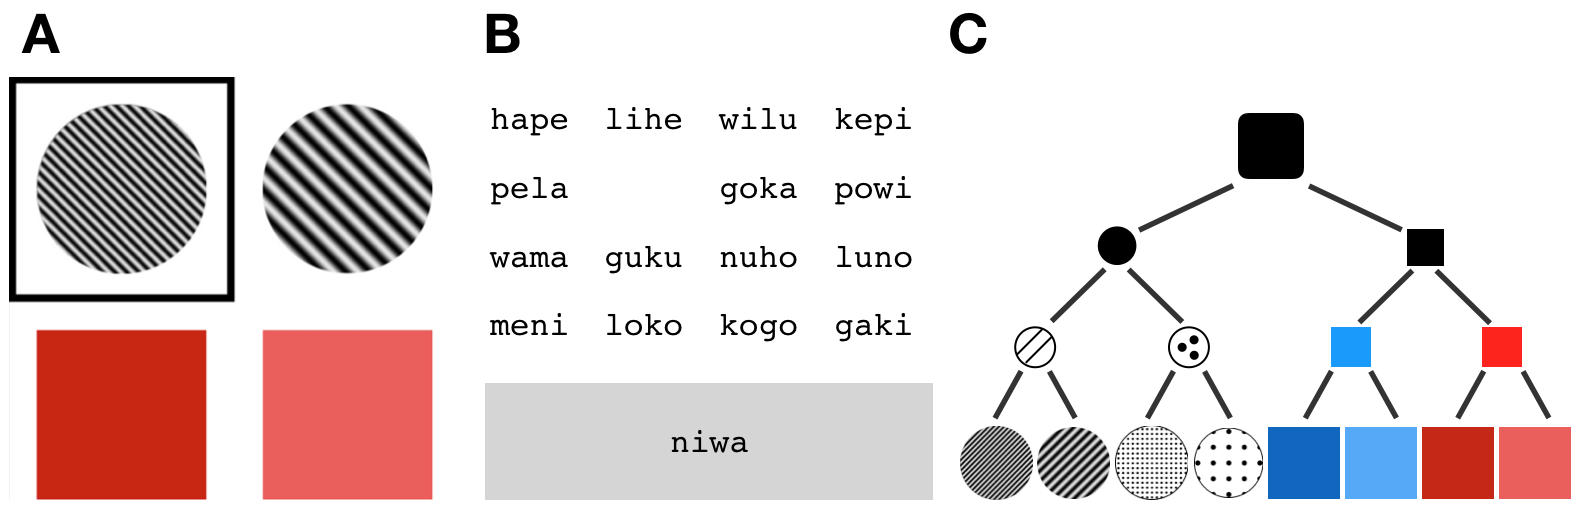
\includegraphics[scale=.55]{./figures/Sec2-design.png}}
{\caption{{(A) Example of \emph{fine} context where one of the distractors belongs to the same fine-grained branch of the hierarchy as the target (i.e.\ another striped circle), so any abstract label would be insufficient to disambiguate them. The target is highlighted for the speaker with a black square. (B) Drag-and-drop chat box interface. (C) Hierarchical organization of stimuli.\label{fig:context_design}}}}
\vspace{-2ex}
\end{center}
\end{figure*}

In the previous section, we examined a mechanism for rapid, partner-specific learning that allows agents to form stable but arbitrary \emph{ad hoc} conventions. 
While a degree of arbitrariness is central to conventionality -- there must exist more than one solution that would work equally well -- this does not necessarily imply that all possible conventions for a meaning are equally likely in practice, or even that all meanings are equally likely to become conventionalized in the first place \cite{HawkinsGoldstone16_SocialConventions}.

For example, while most English speakers have the basic-level word ``tree'' in their lexicon, along with a handful of subordinate-level words like ``maple'' or ``fir,'' we typically do not have labels exclusively referring to each individual tree in our yard.
If we need to refer to a specific tree, we instead create a referring expression \emph{on the fly.}
Meanwhile, we \emph{do} often have conventionalized labels (i.e. proper nouns) for individual people and places that we regularly encounter in our daily lives.
Why do conventions form at some levels of abstraction rather than others?
Here, we show how our proposed theory accounts for these key patterns of \emph{context-sensitivity} as arising naturally from communicative need in dyadic interaction.

In particular, functional accounts of linguistic conventions have frequently observed that lexical systems are well-calibrated to the statistics of the environment \cite{gibson2019efficiency}.
This ``optimal expressivity'' hypothesis has accounted well for the lexical distributions found in natural languages across semantic domains like color words and kinship categories \cite{KempRegier12_KinshipCategories,regier201511,gibson2017color,kemp2018semantic}, as well as the compositional systems that emerge under iterated learning with communication in the lab \cite{WintersKirbySmith14_LanguagesAdapt, KirbyTamarizCornishSmith15_CompressionCommunication}. 
For example, languages in warm regions ought to be more likely to collapse the distinction between ice and snow into a single word, simply because there are fewer occasions that require distinguishing between the two \cite{regier2016languages}. 

Thus, while there is abundant evidence for context-sensitivity in the \emph{outcomes} that result from convention formation processes, it is currently unclear what cognitive mechanisms are necessary to give rise to such outcomes.
That is, context-sensitivity has not yet been grounded in a cognitive and mechanistic account of the processes unfolding in the minds of individual agents as they interact.
Our inferential account hypothesizes that local context shapes the conventionalization process through the mechanisms of pragmatic reasoning over the shorter timescales of dyadic interactions.
%While our hypothesis about ad hoc conventionalization specifically concerned the shorter timescales of dyadic interaction, similar pressures may operate over the multi-generational timescales of cultural evolution. %,  operate on the shorter timescales of dyadic interaction. 
%Better understanding the effect of context on local conventions rapidly formed by adaptive agents over extended interactions may therefore be valuable for understanding how \emph{languages} are globally shaped by communicative constraints.
%Recent computational approaches to language evolution have argued that the lexical conventions of languages balance simplicity, or learnability, with the communicative needs of their users over longer timescales. 
%% Hypothesis
%Under the logic of a local efficiency/informativity tradeoff, we make two predictions about the emergence of abstractions in dyads. 


First, we fill a gap in the empirical literature by collecting a new dataset of human interactions under different environmental statistics.
This experiment manipulates the context of distractors in a repeated reference game where participants must interactively coordinate on an artificial language from scratch. %\cite<e.g.>{GalantucciGarrod11_ExperimentalSemiotics}.
% which allows us to examine the conventions that form in different communicative contexts.
Second, we compare different model predictions by reporting simulations of artificial agents interacting in the same contexts.
In both the empirical data and simulations, we find that conventions come to reflect the distinctions that are functionally relevant for communicative success. 
Furthermore, we find that pragmatic reasoning is necessary for these effects to arise. 
%% Example that sets up our specific hypothesis?

%Suppose, mixing thought experiments from \citeA{Wittgenstein09_PhilosophicalInvestigations} and \citeA{Quine13_WordAndObject}, that two travelers meet in a forest, with no language in common. One is cooking dinner, and the other agrees to help in exchange for food and shelter. What kind of micro-language do they coordinate on to solve this joint task, and how is it shaped by context? 
			
\subsection{Experimental methods}

\subsubsection{Participants}

We recruited 278 participants from Amazon Mechanical Turk to play an interactive, multi-player game using the framework described in \citeA{Hawkins15_RealTimeWebExperiments}. Pairs were randomly assigned to one of three different conditions, yielding between $n=36$ and $n=53$ dyads per condition, after excluding participants who disconnected before completion.\footnote{All materials and data are available at \url{https://github.com/hawkrobe/conventionalizing_hierarchies}; planned sample sizes, exclusion criteria, and behavioral analysis plan were pre-registered at \url{https://osf.io/2hkjc/}.}

\subsubsection{Procedure \& Stimuli}
Participants were paired over the web and placed in a shared environment containing an array of objects (Fig.\ \ref{fig:context_design}A) and a `chatbox' to send messages from a randomly generated vocabulary (Fig.\ \ref{fig:context_design}B). On each of 96 trials, one player (the `speaker') was privately shown a highlighted target object and allowed to send a single word to communicate the identity of this object to their partner (the `listener'), who subsequently made a selection from the array. Players were given full feedback, swapped roles each trial, and both received bonus payment for each correct response.

The objects that served as referents were designed to cluster in a fixed three-level hierarchy with shape at the top-most level, color/texture at the intermediate levels, and frequency/intensity at the finest levels (see Fig.\ \ref{fig:context_design}C). Each communicative context contained four objects. Distractors could differ from the target at various level of the hierarchy, creating different types of contexts defined by the finest distinction that had to be drawn. We focus on two: \emph{fine} trials, where the closest distractor belongs to the same fine-grained subordinate category (e.g.\ another striped circle; see Fig.\ \ref{fig:context_design}A), and \emph{coarse} trials, where the closest distractor belongs to a coarser level of the conceptual hierarchy (e.g.\ dotted circle instead of striped circle).\footnote{Even coarser trials with super-ordinate distractors (e.g.\ a circle target among three square distractors) were logically possible but would have introduced several experimental confounds; we opted to leave these trial types out of our design and conduct the minimal manipulation.} Fixed arrays of 16 utterances (enough to allow the potential for full expressibility) were randomly generated for each pair (and held constant across trials) by stringing together consonant-vowel pairs into pronounceable 2-syllable words (see Fig.\ \ref{fig:context_design}B).

Critically, we manipulated the statistics of the context in a between-subjects design to test the context-sensitivity of conventions. 
In the pure \emph{fine} and \emph{coarse} conditions, all targets appeared in fine or coarse contexts, respectively.
In the \emph{mixed} condition, the two context types were equally likely. 
Sequences of trials were constructed by randomly shuffling targets and trial types within blocks and ensuring no target appeared more than once in a row. 
In addition to behavioral responses collected over the course of the game, we designed a post-test to explicitly probe players' final lexica. For all sixteen words, we asked players to select all objects that a word can refer to (if any), and for each object, we asked players to select all words that can refer to it (if any). 
This bidirectional measure allows us to check the internal validity of the lexica reported.

\subsection{Behavioral results}

\subsubsection{Partners successfully learn to communicate}

Although participants in all conditions began with no common basis for label meanings, performing near chance on the first trial (proportion correct $= 0.19$, 95\%~CI~$=~[0.13, 0.27]$), most pairs were nonetheless able to coordinate on a successful communication system over repeated interaction (see Fig.\ \ref{fig:context_accuracy}). 
A mixed-effects logistic regression on listener responses with trial number as a fixed effect, and including by-pair random slopes and intercepts, showed a significant improvement in accuracy overall, $z = 14.4, p < 0.001$. 
Accuracy also differed significantly \emph{across} conditions (Fig.\ \ref{fig:context_accuracy}): adding an additional main effect of condition to our logistic model provided a significantly better fit, $\chi^2(2) = 10.8, p = 0.004$. 
Qualitatively, the \emph{coarse} condition was easiest for participants, the \emph{fine} condition was hardest, and the \emph{mixed} condition was roughly in between. % Looking more closely at games within the mixed condition, we found that performance on subordinate and intermediate trial types roughly mirrored the gap between the .
Finally, the (log) response time taken by the speaker to choose an utterance also decreased significantly over the course of the game, $t = -19.7, p < 0.001$, indicating that lexical mappings became increasingly established or accessible.

\begin{figure}[t]
\begin{center}
{\includegraphics[scale=0.63]{./figures/accuracyByCondition_edited.pdf}}
%{\includegraphics[scale=.64]{lexiconSize.pdf}}
{\caption{{Players learn to coordinate on a successful communication system. Each point is the mean proportion of correct responses by listeners; curves are nonparametric fits.  %\todo[inline]{rdh questions: Use semantically meaningful condition codes, e.g.\ red/blue/purple? Is this too far aggregated from data (e.g.\ show error bars on each point? fit curves to individual-level binary responses instead of through group means?)}  
\label{fig:context_accuracy}}}}
\vspace{-3ex}
\end{center}
\end{figure}


\begin{figure*}[t]
\begin{center}
\includegraphics[scale=0.75]{Sec2-results.pdf}
\caption{Pragmatic demands of context shape the formation of abstractions. (A) Mean number of words participants reported with specific meanings (applying to 1 object) or abstract meanings (applying to 2 objects). (B) Diversity of terms within reported lexica: many participants in the \emph{coarse} condition reported a mixture of abstract and specific terms.}
%Each participant provided meanings for all sixteen words in their vocabulary box (including selecting no objects if it had no meaning). 
%In the \emph{coarse} condition, participants reported fewer total words in their vocabulary and more of the words they did have were abstractions applying to more than one object. %Distribution of extension sizes in lexica reported across conditions, including those with no extensions  
%\todo[inline]{KS: You'll have to explain how a word can have no extensions, but I'd be tempted to not show these in these graphs? Assuming these are uninteresting (?), showing proportion of  1 vs more-than-1 object words would make the result much clearer. Do you have this in to also show the lexicon size difference? Could show that more straightforwardly with a plot of number of words poer condition?} . 
%Nearly every word reported in the \emph{fine} condition referred to a single object and the \emph{mixed} condition is more similar to the \emph{fine} condition than the \emph{coarse} condition.
%(B) Diversity of terms within reported lexica: many participants in the \emph{coarse} condition reported a mixture of abstract and specific terms.% \todo[inline]{TODO: A/B labels; use \# words instead of \%; change axis labels in B to `'' and ``\# words referring to multiple objects'';}  
\label{fig:lexiconContent}
\end{center}
\end{figure*}


\subsubsection{Partners converge on similar conventions}

Another indicator of successful learning is convergence or alignment of lexica across partners in a dyad. Before using post-test responses to compute similarity \emph{across} partners, however, we examine the internal consistency \emph{within} an individual's post-test responses. For each participant, we counted the number of mismatches between the two directions of the lexicon question (e.g.\ if they clicked the word `mawa' when we showed them one of the blue squares, but failed to click that same blue square when we showed `mawa'). In general, participants were quite consistent: out of 128 cells in the lexicon matrix (16 words $\times$ 8 objects), the median number of mismatches was 2 (98\% agreement), though the distribution has a long tail (mean $= 7.3$). We therefore conservatively take a participant's final lexicon to be the \emph{intersection} of their word-to-object and object-to-word responses.

Using these estimates of each participant's lexicon, we compute the overlap between partners. For most pairs, partners aligned strongly by the end, with a median post-test overlap of 97.6\% (125 out of 128 entries). Because these matrices were extremely sparse, however, just a a few mismatches could have a large impact on performance. Overall accuracy in the game is strongly correlated with alignment: partners who reported more similar lexica at the end tended to perform better at the task ($r = 0.77$).  

Despite these markers of success at the group level, individual performance was bimodal: a subpopulation of 29 games (11\% of coarse games, 18\% of mixed, and 39\% of fine) still showed relatively poor performance, sometimes at chance, by the end of the game. For the subsequent analyses focusing on the content of the lexicon, we exclude games with fourth-quartile accuracy below the pre-registered criterion of 75\% to ensure we are examining only successful lexica. %After removing these participants, internal consistency was roughly similar across conditions (means of 3.0 and 3.4 internal mismatches in the \emph{coarse} and \emph{fine} conditions, and 5.8 in \emph{mixed}) so we don't expect these to bias our data.

\subsubsection{Contextual pressures shape the lexicon}

We predicted that in contexts regularly requiring speakers to make fine distinctions among objects at subordinate levels of the hierarchy, we would find lexicalization of specific terms for each object (indeed, a one-to-one mapping may be the most obvious solution in a task with only 8 objects). Conversely, when no such distinctions were required, we expected participants to adaptively lexicalize more abstract terms. One coarse signature of this prediction lies in the \emph{efficiency} of the resulting lexicon: lexicalizing abstract terms should require participants to use fewer terms overall.

To test this prediction, we counted the number of words in each participant's reported lexicon (i.e.\ the words for which they marked at least one object in the post-test). We found that participants in the \emph{coarse} condition reported significantly smaller, more efficient lexica ($m = 4.9$ words) than participants in the \emph{mixed} and \emph{fine} conditions ($m = 7.4, t = 10.3, p <0.001$ and $m = 7.6, t = 9.5, p < 0.001$, respectively; see Fig.\ \ref{fig:lexiconContent}A). At the same time, the smaller lexicon provided equivalent coverage of objects: the median number of objects where participants agreed on the same word or words was 7, 6.5, and 7, respectively. 


If participants in the \emph{coarse} condition can get away with fewer words in their lexicon, what are the meanings of the words they do have? We counted the numbers of `specific' terms (e.g.\ words that refer to only one object) and `abstract' terms (e.g.\ words that refer to two objects) in the post-test. We found that the likelihood of lexicalizing abstractions differed systematically across conditions (see Fig.\ \ref{fig:lexiconContent}A). Participants in the \emph{fine} condition reported lexica containing exclusively specific terms, while participants in the \emph{coarse} condition reported significantly more abstract terms ($m = 2.5, p < 0.001$). 

These data also reveal an interesting asymmetry in lexicon content across conditions: while abstractions are entirely absent from the \emph{fine} condition, participants in the other conditions often reported a mixture of terms (see Fig.\ \ref{fig:lexiconContent}B). In the \emph{coarse} condition, for instance, participants could in principle perform optimally with only four abstract terms and no specific terms. While this was the modal system that emerged (reported in the post-test by nearly 1/3 of participants), the average proportion of abstract (vs.\ specific) terms \emph{within} each participant's lexicon in the \emph{coarse} condition ($m = 0.56$) was significantly higher than in the other conditions ($p < 0.001$, exploratory).

\subsection{Simulation results}

Our empirical results suggest that different communicative contexts systematically lead to different communicative conventions.
Critically, the sequence of targets was held constant across the \emph{course}, \emph{fine}, and \emph{mixed} conditions; only the distractors were manipulated.
In this section, we show how our model explains such sensitivity as the consequence of pragmatic reasoning \cite<e.g.>{GoodmanFrank16_RSATiCS,FrankeJager16_ProbabilisticPragmatics} over a space of taxonomic word meanings \cite{XuTenenbaum07_WordLearningBayesian}.

This task poses several distinct challenges for models of coordination and convention formation.
First, the context constantly changes, with a subset of only four of the eight total objects shown on each trial.
Second, the stimuli are embedded in a conceptual taxonomy, where some objects are more similar than others.
These 

Here we must consider a space of meanings that reflects the conceptual structure of the stimulus hierarchy. 
That is, in addition to 8 meanings at the sub-ordinate level (one for each individual object), we populate the hypothesis space with 4 meanings at the basic-level (striped, spotted, blue, red), 2 meanings at the super-ordinate level (circle and square) and 1 exhaustive meaning (shape).

 
 \todo[inline]{New additions: (1) memory discounting, (2) mutual exclusivity, (3) discrete space of taxonomic meanings vs. independent real-valued lexicon, (4) addition of pure truth term}
\todo[inline]{the non-pragmatic version seems to converge to a degenerate 2-word (cricle/squre) state (initial usage is ambiguous b/w levels, so someone will eventually extend to different object, then only way to accomodate that data is to rule out more specific meanings). if we allowed a degenerate meaning where all words have same meaning, it would converge to that; can't tell that it's confusing and is guaranteed to be literally true!}
\todo[inline]{May need to implement baseline model from other papers (e.g. Steels-style, or Spike implementation?) rather than using this version, since it has somewhat different behavior, I think.}

\todo[inline]{Make a note that in the limit it doesn't matter whether you have pragmatics in both learning rule or decision rule. In case where it's only in production rule, you'll produce the data with the necessary biases in learning.}

\todo[inline]{First, show theoretical guarantees of lexical systems that arise when models condition on the same data with and without pragmatics?}
\todo[inline]{Second, show that we can also capture learning curves if we introduce memory discounting, etc.?}


\todo[inline]{Explain simulation details; for each dyad in our human-human dataset, we pair up two artificial agents. They update based on previous choices, etc...}
We use these pragmatic speaker and listener likelihood functions to link latent lexica, represented as a matrix of real values $\ell_{w,o}^t \in \mathbb{R}$, to behavior.
Because each trial has only a single choice for each player, we pool statistics within $k$ epochs of the data (we choose $k=6$ such that each target appears exactly twice in each epoch). 
As in our earlier simulations, we sample lexical entries from independent Gaussian priors: $$\ell_{o,w}^k\sim\mathcal{N}(0, 5)$$ 
We approximate the posterior of this model separately for each pair using mean-field variational inference, implemented in the probabilistic programming language WebPPL \cite{GoodmanStuhlmuller14_DIPPL,DAIPP}. 
The approximating family for each random variable is Gaussian.

%\begin{figure*}[t]
%\begin{center}
%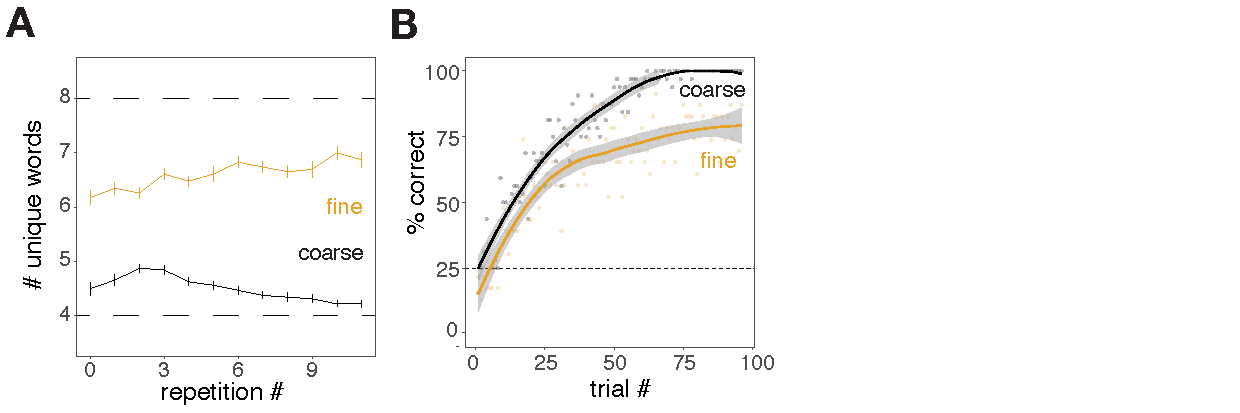
\includegraphics[scale=0.7]{./figures/sec2-modelFig.pdf}
%\vspace{-1ex}
%{\caption{{Model-based results. (A) A logistic classifier based on inferred lexical entries accurately predicts post-test responses. (B) Entropy of posterior word extensions show coalescence across epochs for each condition. (C) Mean change in entropy at the word level from trial to trial (error bars are $\pm 1$ SE)}  \label{fig:postTestPrediction}}}
%\end{center}
%\vspace{-3ex}
%\end{figure*}
\todo[inline,caption={}]{Tom: there are a few moving parts that I am currently exploring:
\begin{enumerate}
\item We need to say what happens after an unsuccessful communication attempt. Currently, speaker and listener are conditioning on different data (speaker conditions on what listener chose; listener conditions on what speaker said), which leads to persistent mis-coordination even later in the game. 
\item We may just need a simple mechanism for forgetting. According to Spike et al., 2018 this is necessary for convergence. the problem is that random guesses at the beginning of the interaction will confuse agents much later: even at the end, they'll continue to think that 4 different words can possibly refer to the same object even if only a single one has ever successfully referred to it. We're amortizing inference anyway, so maybe we should try just updating on most recent 16 trials or something?
\item another idea is to design some inductive bias for the likelihood that weights 'successes' as stronger evidence than 'failures'... but this seems unmotivated.
\item another question is whether to sample vs. using a MAP decision rule when running agents forward
%\item inductive biases for certain levels of hierarchy? (e.g. some levels weighted more strongly?)
\end{enumerate}
}
\subsection{Discussion}

Previous proposals have handled context-sensitivity in different ways.
In some common settings for convention formation, there is no explicit representation of context at all, as in the task known as the ``Naming Game'' where agents coordinate on names for objects in isolation \cite{Baronchelli,oldnaminggame}. 
In other common settings, context is central but held constant throughout interactions, as in Lewis signaling games, where agents use a fixed set of messages to communicate a fixed set of world states \cite{lewis,signalinggame}.
One of the most sophisticated studies of context in prior work is the Discrimination Game of \citeA{steels2005coordinating}, which examined the joint formation of color categories and color naming conventions.
As in our experiments, contexts were generated randomly on each trial from a large space and stimuli are embedded in a similarity space (with similarity based on Euclidean distance in continuous space rather than taxonomic relations).
Unlike our task, contexts were not systematically manipulated, and the resulting level of abstraction was not evaluated: the only restriction was to ensure that color chips were a fixed minimum distance apart.

In models using Roth-Erev reinforcement learning update rules or simple neural networks, the referential context is sometimes accounted for with a \emph{lateral inhibition} heuristic used by both the speaker and listener agents \cite{franke2012bidirectional}.
If communication is successful, the connection strength between the label and object is not only increased, the connection between the label and competing objects (and, similarly, between the object and competing labels) is explicitly \emph{decreased} by a corresponding amount \cite<see also>{steels2005coordinating}.
This lateral inhibition heuristic is functionally similar to our pragmatic reasoning mechanism, in terms of allowing the agent to learn from negative evidence (i.e. the speaker's choice \emph{not} to use a word, or the listener's choice \emph{not} to pick an object). 
Under an inferential framework, however, this property emerges as a natural consequence of well-established Gricean principles of pragmatic reasoning.
As previously observed by \cite{FrankGoodmanTenenbaum09_Wurwur} in the context of early cross-situation word learning, reasoning about speakers' intentions naturally instantiates a kind of inductive bias for \emph{mutual exclusivity}.


%\subsection{Validating post-test responses}
%
%We begin by showing that the lexical entries we infer for each participant accurately predict their post-test responses. 
%We constructed a logistic classifier from our posterior on each epoch: for each object-word pair $(o,w)$ in the post-test response matrix, we computed the marginal posterior probability $P(\ell_{o,w} > 0.5| \theta_{o,w})$, where $\theta_{o,w}$ are the corresponding variational parameters (i.e. the mean and variance of the approximating Gaussian). This gives the posterior probability that word $w$ applies to object $o$. We evaluated the performance of this classifier by constructing an ROC curve that shows the tradeoff between hits and false alarms as the discrimination criterion is varied. We found that the classifier based on the final epoch predicts post-test responses with excellent accuracy (AUC: $0.98$; see Fig.\ \ref{fig:postTestPrediction}A). This indicates that the post-test lexicon is indeed linked to behavior as predicted by RSA, validating both the post-test measure and the results of our Bayesian analysis.
%
%Furthermore, we found that the corresponding posterior predictives from earlier epochs predicted final post-test responses less well, even though they were learned from the same number and type of behavioral observations (Fig.\ \ref{fig:postTestPrediction}A). Still, even the classifier based on the earliest epoch performs above chance, indicating that some information about the final lexicon is available from the earliest trials. These patterns are suggestive of a path-dependent process where the lexicon gradually coalesces from initially arbitrary associations over the course of interaction. We next turn to the earliest stages of this process.% to examine this process in more detail.
%
%\subsection{Examining early time course}
%
%%\todo[inline]{note for MF: I got this feature-based model working and then Noah thought it might be better to just use the simple model for everything? I'm going to see how far I can run with the simple model, so this section is somewhat in flux\dots}
%
%%Classic theories in historical linguistics distinguish between semantic \emph{broadening}, when a word takes on a more inclusive meaning, and \emph{narrowing}, when meanings become more restrictive over time \cite{TraugottDasher02_RegularitySemanticChange}. 
%One advantage of the statistical approach we develop here is the ability to make descriptive inferences about the meanings being used in settings where we \emph{don't} ask participants for explicit judgements---in particular, in early trials of our games. 
%
%Our primary measure of interest is the \emph{entropy} of the extension of words over the eight objects. The entropy of a particular word is near zero when its meaning is peaked on a single object, and is maximized when could apply equally to all objects (e.g. for a novel word that has not yet been used). 
%%In principle, we would find uniform distributions for words that apply equally well to all eight objects, but in our case, uniform meanings are more likely to reflect the uncertainty in our model's posterior (e.g. for words that were never used in a game). 
%We expect abstract terms to lie in between these extremes. 
%We obtain the extension distribution for each word by running it through our $L_0$ model, essentially asking how likely it is to refer to each of the eight objects.\footnote{Using $L_0$, rather than $L_1$ or $\mathcal{L}$, gives us a notion of word extension that is close to the underlying lexicon while influenced by non-identifiability of parameters. For instance, $\mathcal{L}$ has an overall scaling per row that doesn't influence behavior.} 
%We use the MAP estimate of the lexicon. % (in order to make entropy effects more evident). 
%The resulting distribution of estimated word entropies, aggregated for each epoch and condition, is shown in Fig. \ref{fig:postTestPrediction}B. %There are two properties to note here. 
%Abstract terms begin to form early (epoch 2) in the \emph{coarse} condition, and remain stable throughout the game. In contrast, specific terms are relatively slow-forming (epoch 4-5) in the other two conditions. The peak near an entropy of 3 reflects the inferred ambiguity of words that were not used or used randomly.
%
%Because these distributions are aggregated across words, however, they leave open the possibility that lexica are not stabilizing or coalescing but simply cycling through different words each epoch. We address these dynamics more thoroughly at the \emph{word} level by computing the difference in each word's entropy from epoch to epoch (Fig. \ref{fig:postTestPrediction}C). For all conditions, we found that the entropy of individual words changed less over later epochs (i.e. the difference scores approached zero), indicating that meanings gradually stabilized. There are also differences across conditions: words in the \emph{mixed} and \emph{fine} condition began with high entropy reduction (becoming more specific) which continued through the final epochs, while words in the \emph{coarse} condition actually seemed to increase in entropy across the game on average.
%These preliminary results, then, may reflect a combination of narrowing and broadening depending on condition. Unknown words can initially refer to any of the objects and only acquire more informative meanings as agents learn through interaction. Yet in the coarse condition where agents are quick to adopt meanings, the rest of the game may be spent paring down the lexicon instead.

%\ndg{i think we should try to squeeze in a figure for the entropy differences...}

%For this analysis, we elaborated our model to use an underlying feature basis to derive the lexicon instead of independent entries for each object-word combination. 
%\ndg{can't we first do this analysis using the simple lexicon model? }
%That is, we re-encoded each of the eight objects as a point in a discrete seven-dimensional feature space roughly corresponding to the nodes of the hierarchy\footnote{(shape, red-ness, blue-ness, stripe-ness, spot-ness, pattern frequency, and color intensity)} and learned an embedding for each word in this space. The meaning function used by our literal listener, then, is simply $L^2$ similarity between the word and object vectors. This feature-based representation has two useful properties. First, it allows for more meaningful feature-based generalization: having observed a word associated with one red square, it is more likely to extend this term to the other red square than to a striped circle simply because of their relative distances in the space. Second, it provides a way to directly read out more abstracted terms from the inferred lexicon (e.g.\ by looking at whether the red-ness feature is high and the brightness term is at the mid-point). 

%The mixed pairs can get by with their lexicon of specific terms, and even the coarse pairs are stuck with the residue of their early specific terms. 

%\todo[inline]{TODO: use simple model to look at the expected extension size of each word, and how it changes between quartiles.... walk through examples of early rounds in different contexts; show timecourse of abstractions, e.g.\ are initially specific terms extended or are initially abstract terms narrowed?  Do you tend to move from big to small or small to big quarter-to-quarter?}



% For an example of a full page figure, see Fig.~\ref{fig:myFullPageFigure}.

